\section{命令行}

\begin{frame}[t]{基本操作}
    \centering
    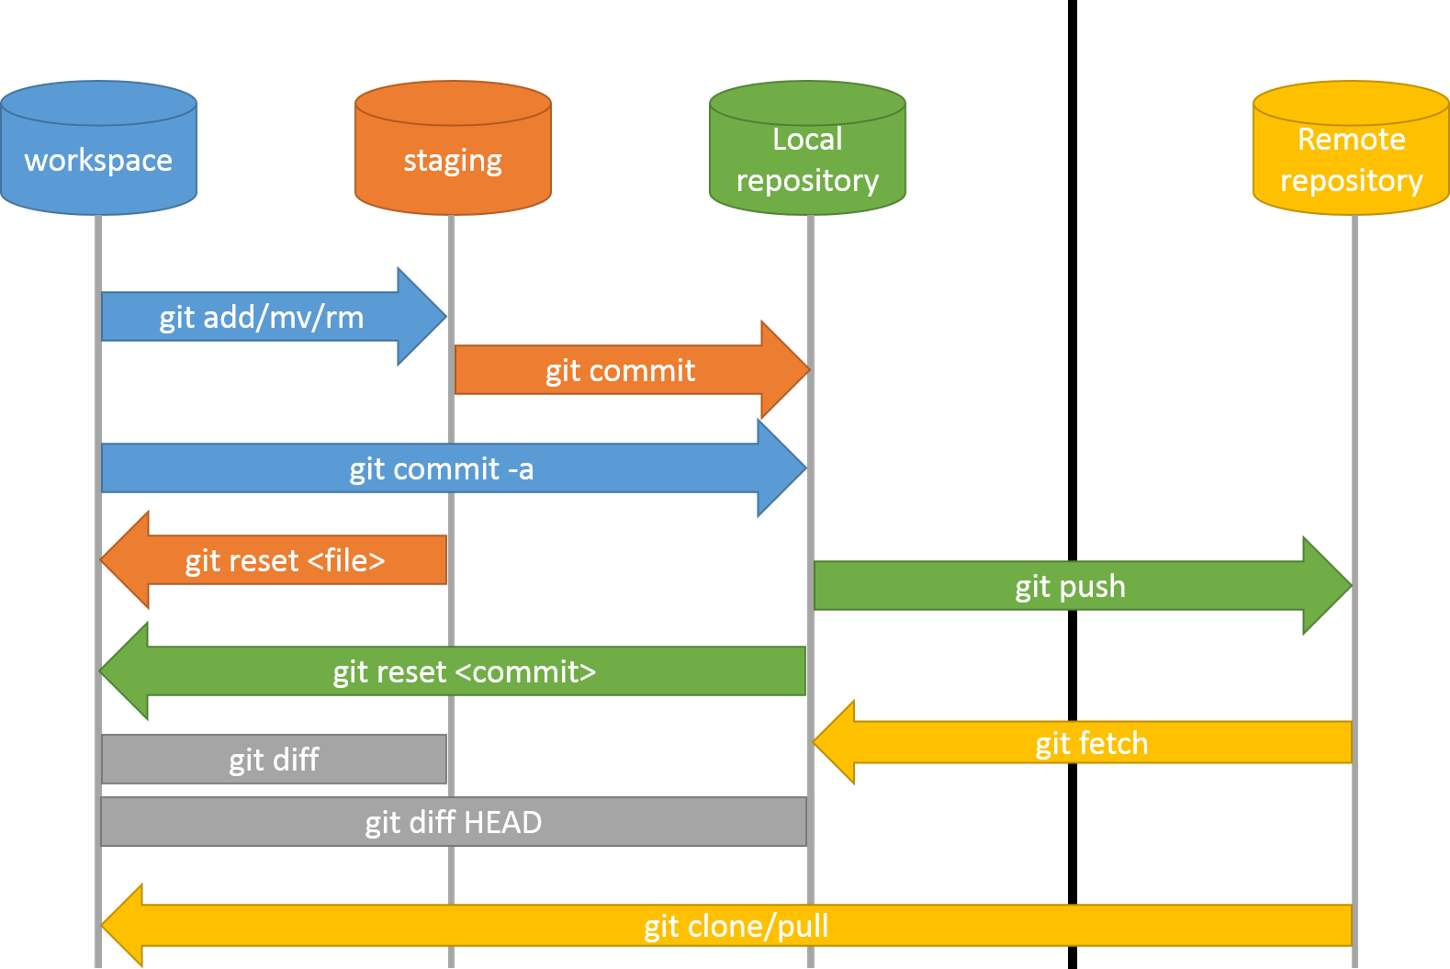
\includegraphics[scale=0.38]{figures/git-basic.jpg}
\end{frame}

\begin{frame}{操作\en{Svn}}
    \centering
    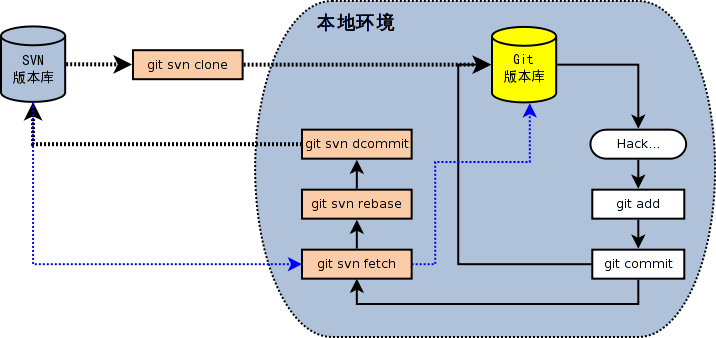
\includegraphics[scale=0.42]{figures/git-svn-basic.jpg}
\end{frame}

\begin{frame}[fragile]{其它常用操作(一)}
    \begin{lstlisting}
        # 查看分支
        git branch -a
        # 切换至指定分支
        git chekcout <BranchName>
        # 基于当前分支创建并切换至新分支
        git checkout -b <BranchName>
        # 合并整个目标分支至当前分支
        git merge --no-ff <BranchName>
        # 合并指定的单次提交至当前分支
        git cherry-pick <CommitID>
        # 删除本地分支
        git branch -D <BranchName>
        # 重命名本地分支
        git branch -m <OldName> <NewName>
    \end{lstlisting}
\end{frame}

\begin{frame}[fragile]{其它常用操作(二)}
    \begin{lstlisting}
        # 添加远程仓库地址
        git remote add <RemoteName> <RemoteAddr>
        # 修改远程仓库地址
        git remote set-url <RemoteName> <RemoteAddr>
        # 删除远程仓库地址
        git remote remove <RemoteName>
        # 删除远程分支
        git push --prune <RemoteName> <RemoteBranch>
        # 创建新标签
        git tag <TagName> <BaseCommitID>
        # 删除标签
        git tag --delete <TagName>
        # 推送本地标签至远程仓库
        git push --tags
    \end{lstlisting}
\end{frame}

\begin{frame}[fragile]{其它常用操作(三)}
    \begin{lstlisting}
        # 基于指定的起点,重新整理提交记录
        git rebase -i <BranchName>
        # 将所有未提交的更改收入隐藏区(垃圾桶)
        git stash
        # 清理所有未纳入版本库管理的文件与目录
        git clean -fdx
        # 查看近期所有分支上的操作日志
        git reflog
        # 查看内容有变动的文件列表
        git diff --name-only <BranchName>
        # 子模块递归更新
        git submodule update --init --recursive
        # 定义指令别名
        git config --global alias.<Alias> <SubCMD>
    \end{lstlisting}
\end{frame}